% CVPR 2022 Paper Template
% based on the CVPR template provided by Ming-Ming Cheng (https://github.com/MCG-NKU/CVPR_Template)
% modified and extended by Stefan Roth (stefan.roth@NOSPAMtu-darmstadt.de)

\documentclass[10pt,twocolumn,letterpaper]{article}
\usepackage{cvpr}

% Include other packages here, before hyperref.
\usepackage{graphicx}
\usepackage{amsmath}
\usepackage{amssymb}
\usepackage{booktabs}
\usepackage{subcaption}
% It is strongly recommended to use hyperref, especially for the review version.
% hyperref with option pagebackref eases the reviewers' job.
% Please disable hyperref *only* if you encounter grave issues, e.g. with the
% file validation for the camera-ready version.
%
% If you comment hyperref and then uncomment it, you should delete
% ReviewTempalte.aux before re-running LaTeX.
% (Or just hit 'q' on the first LaTeX run, let it finish, and you
% should be clear).
\usepackage[pagebackref,breaklinks,colorlinks]{hyperref}

% Support for easy cross-referencing
\usepackage[capitalize]{cleveref}
\crefname{section}{Sec.}{Secs.}
\Crefname{section}{Section}{Sections}
\Crefname{table}{Table}{Tables}
\crefname{table}{Tab.}{Tabs.}

\begin{document}

\title{Pixel Gradients for Color Invariant Image Classification and Synthesis}

\author{Cole Dilanni \\
{\tt\small diianni@wisc.edu}
\and
Spencer Schoenberg \\
{\tt\small spencer.schoenberg@wisc.edu}
\and
Connor Bailey \\
{\tt\small cbailey9@wisc.edu}
}
\maketitle

\begin{abstract}
    Most machine learning models struggle with color-object entanglement. A model trained on one set of images often learns to associate the objects in that training set with their colors. This means that any bias in the color of objects in the training set will be learned, and any novel-colored objects during test time can confound the model. While models such as convolutional neural networks (CNNs) are translation invariant, there do not exist any similarly color invariant models. In this work, we modify existing model architectures to promote color invariance, which we define as having the same or very similar output when the color of an image is changed without changing the image's semantic meaning. We do this through an architectural change to the first convolution layer in a CNN, removing the direct color values in favor of relative color distances. We first verify the effectiveness of this newly proposed layer by creating classification models and measuring their accuracies. Then, we demonstrate its intuition via a generative adversarial network (GAN). Since our method removes the color information from images, we also develop a colorization algorithm for visualizing the generated images.
\end{abstract}

\section{Introduction}
\label{intro}
Difficulties with color-object entanglement are prevalent in most machine learning models which presents problems for synthesis, manipulation, and classification tasks. One way in which this entanglement is problematic is that models may be biased by the color of objects in the training dataset. For example, a model trained exclusively on red cars may not be able to extrapolate the features it has learned to blue cars. A failure case following the pattern of this example is shown in \Cref{zebras}. Researchers attempt to circumvent any test-time color distribution shift by simply augmenting their training sets with many color-based augmentations. Changes in brightness, lightness, hue, saturation, contrast, normalization, grayscale, jitter, and combinations of these are regularly used to create data augmentations. While this can cover a wide range of color shifts, there is no efficient way to cover the entire space of possible color changes. One naive approach to simulate color invariance is to convert images to grayscale before being passed to a model. As we will show in this paper, using grayscale images can still bias a model. While models such as CNNs are translation invariant, we are unaware of any models which are also color invariant. This stems from the problem of how to define color invariance.

\begin{figure}[h!]
    \centering
    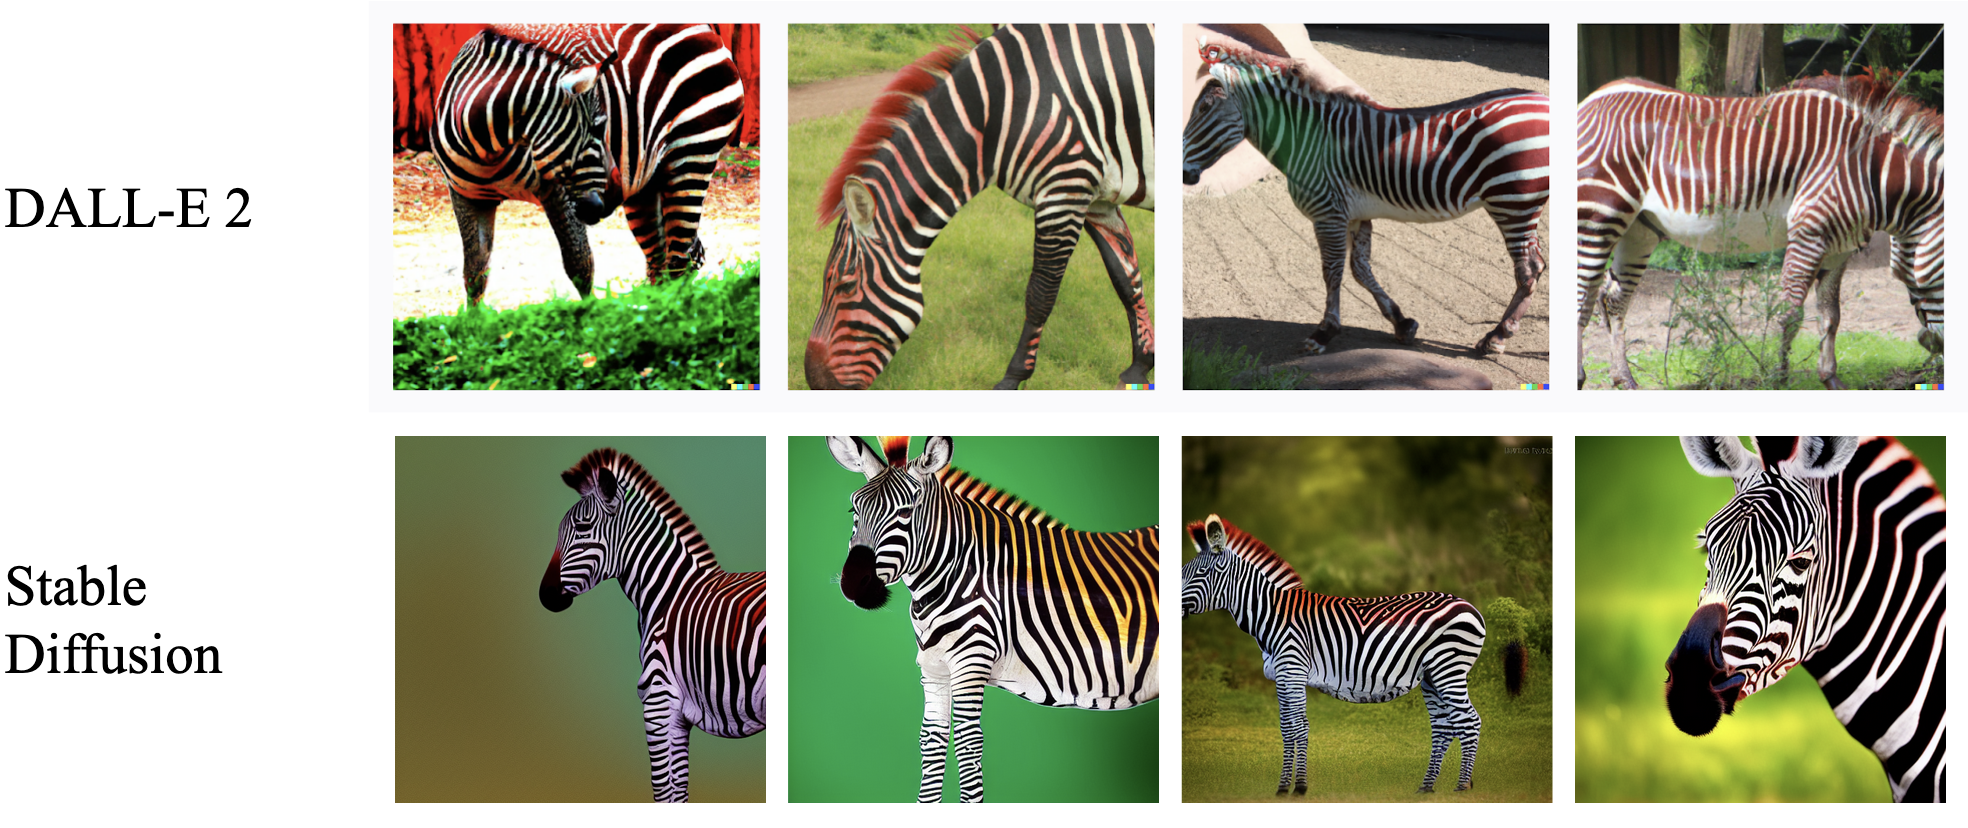
\includegraphics[width=0.48\textwidth]{images/zebras.png}
    \caption{When state of the art diffusion models such as DALL-E 2 and Stable Diffusion are given the prompt of “a photograph of a green and red zebra”, the models cannot disentangle the object and colors. The models have likely learned the black and white stripes are associated with zebras in the training images and therefore fail to produce the desired images for the given prompt.}
    \label{zebras}
\end{figure}

In this work, we consider a model to be color invariant if color changes which do not change an image's semantic meaning have little to no effect on the model's output. For example, a perturbation could change the order of the RGB channels, greatly modifying the color of the image, while keeping the object structure entirely intact. In this work, we modify an existing CNN model architecture to promote color invariance and investigate the implications for how CNNs perceive images. Since only the first convolution layer operates in the image's color space, our architectural changes are confined to the first convolution layer.

We test a modified classification model’s performance on the MNIST and CIFAR-10 datasets to ensure removing the input color values does not drastically harm the model’s performance. A model which lacks color information should be able to focus more on object shape rather than textures, as current CNNs are biased to do \cite{Geirhos18}.

Using the top-performing color distance metric for creating a color invariant convolution layer, we then build a color invariant GAN which generates image gradients rather than RGB values. Given that the GAN does not have specific color values, we hope the generator will learn to focus on generating images with similar semantic meaning to the training dataset. To convert from gradient images to RGB images, we did not want to train an auxiliary model because such a model would require its own training set which would bias the colors of the images. Instead, we employed an iterative gradient descent algorithm to learn an image that has localized gradients which match those of the generated gradient image. This would ensure a coherent local image structure while allowing the overall image color to vary widely. For example, consider training the color invariant GAN on CIFAR-10 horse images which are commonly brown with black manes and black tails. Since the color invariance is local, there is the possibility that the generated gradient images produce a blue horse with a red mane and a green tail when colorized.

\section{Related Work}

There has previously been work comparing different color spaces as input to regular convolutional neural networks \cite{Sachin18}. Similar to this work, we tested the color spaces HSV, LAB, and XYZ in comparison to RGB but did not find significant improvements with any other colorspace and therefore kept our subsequent tests in the RGB space.

Other works investigated illumination invariance \cite{Ng08}\cite{Choi10}\cite{Gevers99}, however illumination invariance does not effectively handle all types of possible color changes in the object. Other works focus on various data augmentations including color changes to make their models more robust to the color-object entanglement problems \cite{Xu22}\cite{Zhang16}, however it is impossible to search over the entire span of possible data augmentations in order to train a color invariant model. These prior works would also likely fail under conditions where the colors of individual parts of an object are changed. The color changes in these works tend to affect entire images at once. In papers that do not just change the color over the whole image, they tend to focus on only one object in each image or one kind of object. Consider again the example of a blue horse with a red mane and a green tail. Classical data augmentation techniques would likely not be able to simulate this object level color perturbation. Yet, a human would still be able to recognize such a horse because the semantic meaning has not changed.

\section{Technical Approach}
In this work, we investigate an architectural change to the convolution layer which promotes color invariance by removing the direct color values. Using this newly proposed layer, we first verify its effectiveness through classification model accuracies and then demonstrate its intuition via a generative model. Since our method removes the color information from images, we also develop a colorization algorithm for generated image visualization.

\subsection{Color Invariant Image Representation}
\label{colorInvariant}
While current convolutional neural networks apply weights directly to RGB values in the first layer \cite{LeCun98}, this can bias their learned filters to focus on detecting certain colors rather than shapes. To remedy this issue, we propose converting the initial layer's RGB input to a pixel-wise distance representation similar to the self-attention used in transformer networks \cite{Vaswani17}. This pixel-wise distance is taken only between the pixels within the kernel receptive field when passing over the image and can be calculated with a variety of distance metrics. In this work, we explore two distance metrics: Euclidean distance and cosine similarity. The Euclidean distance is calculated using \Cref{dist}.

\begin{equation}
    \text{dist}(x_i, x_j) = \sqrt{\sum_{c \in \{R, G, B\}}(x_{i, c} - x_{j, c})^2}
    \label{dist}
\end{equation}

The cosine similarity metric first maps the RGB values of two pixels to a 5-dimensional space using a three layer perceptron and then uses the cosine distance defined in \Cref{cos}.

\begin{equation}
    \cos(x_i, x_j) = \frac{x_i \cdot x_j}{\|x_i \|\|x_j \|}
    \label{cos}
\end{equation}

By using these distance metrics as input rather than the RGB values themselves, any model using the proposed color invariant network will not have access to direct color values, being forced to rely solely on relative color differences to distinguish object structures. By only having access to the pixel-wise distances, our goal is that this technique should bias models toward learning object shapes rather than color. We make the assumption that pixel color similarity should positively correlate with the probability that pixels belong to the same object. We also assume that class labels are independent of object color.

\subsection{Generative Adversarial Network}
A GAN \cite{Goodfellow14} trained with our version of color invariance does not need an architectural change, as the training set images are simply converted to their pixel-wise distance representations and passed into the model. The size of the receptive field is an additional model hyperparameter. The generator learns to generate pixel-wise distance representations, which can later be converted to RGB images using a colorization algorithm. The output pixel-wise distance representation is passed from the generator to the discriminator along with the pixel-wise distance representations of real images.

\begin{figure*}
    \centering
    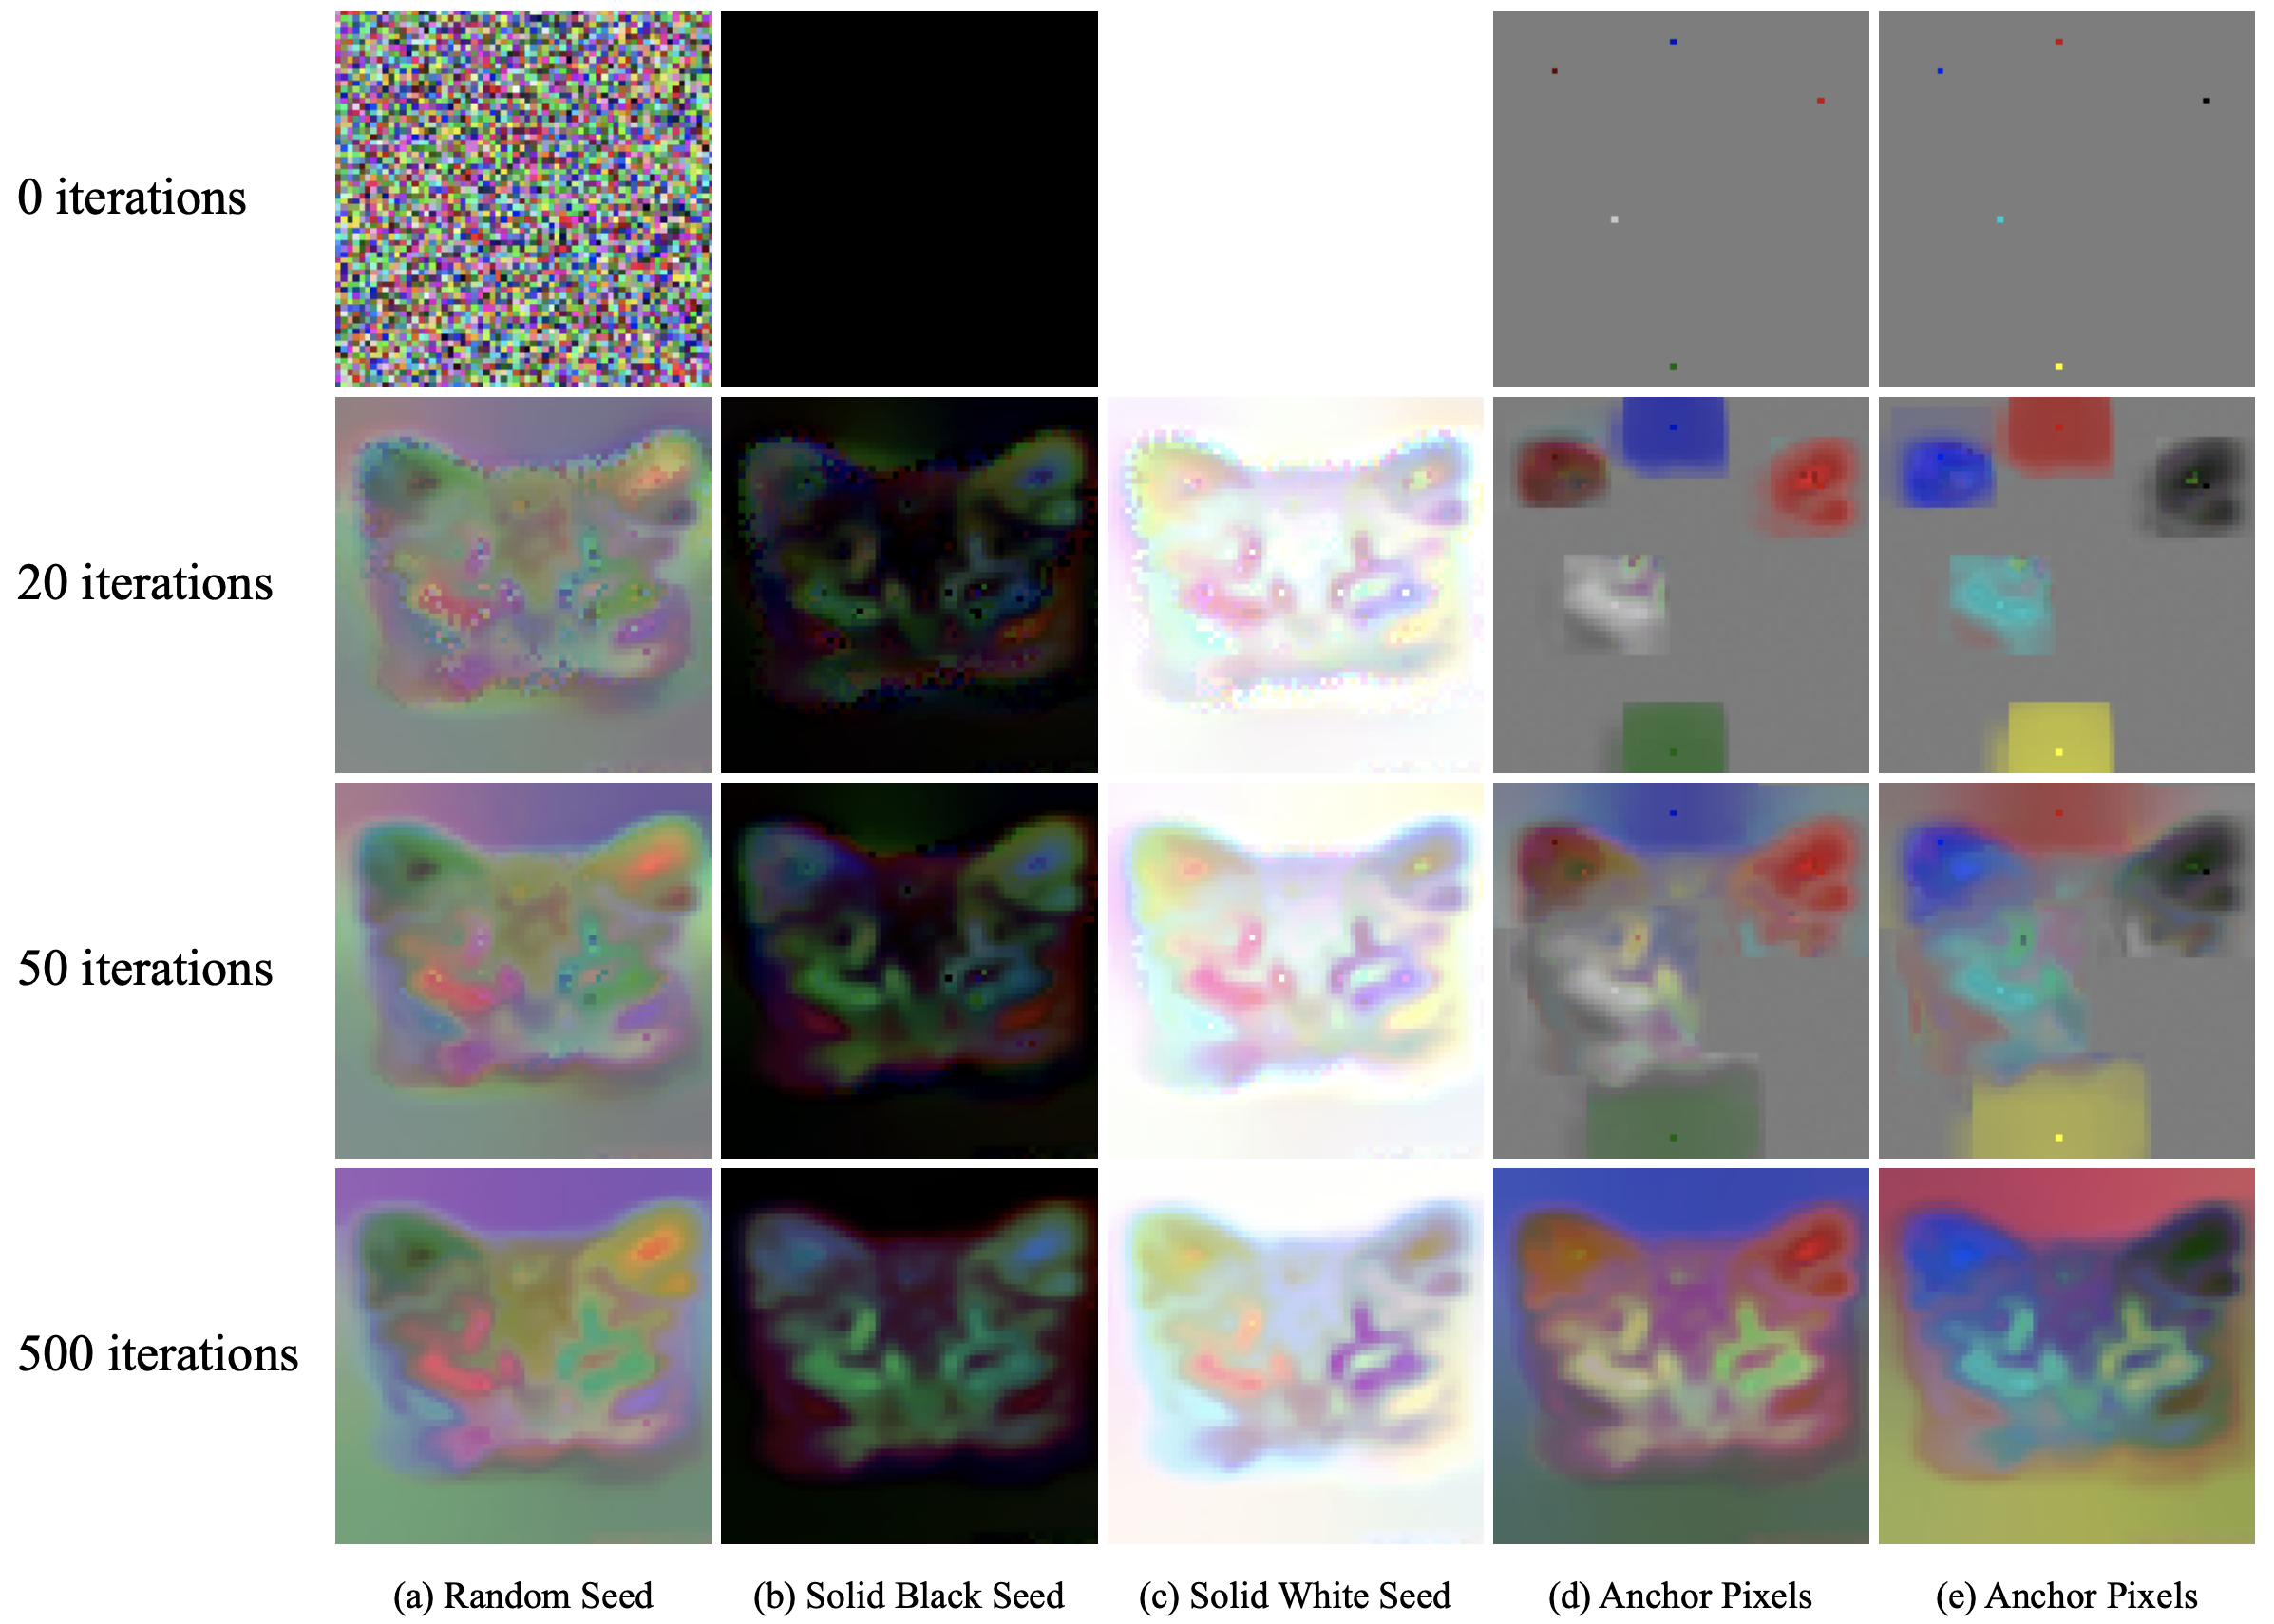
\includegraphics[width=\linewidth]{images/recolorization_grid.png}
    \caption{Colorization algorithm outputs are shown using random seeding (a), solid seeding (b, c), and anchored seeding (d, e) at various iterations. This method uses the original image of a cat to guide the pixel-wise differences such that the local color consistency is maintained while achieving global color invariance. A receptive field of size $9\times9$ was used in this example.}
    \label{recolorization_grid}
\end{figure*}

\subsection{Colorization Algorithm}

To color an image that is formatted as pixel-wise distances, we formulate an optimization problem to find an RGB image that minimizes the $\ell_2$ difference between a starting seed RGB image and the generated pixel-wise distance representation. This is to say we minimize the loss function defined in \Cref{loss}.

\begin{equation}
    \mathcal{L}(x_\text{RGB}, x_\text{PWD}) = \| \text{PWD}(x_\text{RGB}, n) - x_\text{PWD} \|
    \label{loss}
\end{equation}

Where PWD indicates pixel wise distance and $n$ is the size of the receptive field. We solve this problem by developing a novel colorization algorithm which optimizes this loss function by iteratively performing backpropagation with respect to the RGB image. This algorithm takes a given pixel-wise distance representation and subsequently updates the output RGB image's pixels. Each iteration updates the output image to align the pixel-wise distances with the known distances within the $n \times n$ receptive field. During the backpropagation, we also weight the pixel differences based on their proximity within the image to bias the output image's local fidelity. This can be thought of as an altered version of label propagation \cite{Zhu03}, where the image colors are the soft labels, and their weights are dictated by their color and spatial distances. Given this comparison, we show that certain pixels in the starting RGB image can be seeded and then anchored to a particular color, enforcing a color prior on the resulting image as seen in \Cref{recolorization_grid}.

\section{Experiments}
We tested the viability of our color invariant convolution layer on classification tasks using the MNIST \cite{LeCun98} and CIFAR-10 \cite{cifar10} datasets and performed color invariance image synthesis using the CelebA \cite{celeba} dataset.

\subsection{MNIST Classification}
\label{mnistClassification}
We first tested our color invariant convolution layer on the MNIST, handwritten digit classification tasks. For the classification models tested, we start with a basic ResNet-50 model. We remove the normalization because it only applies to RGB inputs. We also remove padding from the first layer to prevent any color information from leaking through our color invariant layer. For example, our layer would be able to determine whether an image border pixel was black if the distances between said pixel and the padded zeros were zero. During this experiment, we tested three models. The first is a base ResNet-50 with only the modifications described above. The second is a ResNet-50 with the first layer converted to our color invariant convolution layer using Euclidean distance as the pixel distance metric. The third is a ResNet-50 with the first convolution layer converted to our color invariant convolution layer using a learned mapping model's cosine similarity (see \Cref{cos}) as the pixel distance metric. All models were trained with a learning rate of 0.1 for a maximum of 300 epochs. To demonstrate a model's ability to generalize to unseen color shifts, we do not use any data augmentation in the training set. We then test on a variety of color-related perturbations shown in \Cref{mnist_perturbations}. Note that the channel drop perturbation randomly inverts the image, then randomly drops up to two channels. This maintains the color difference between the digit and its background.

\begin{figure}[h!]
    \centering
    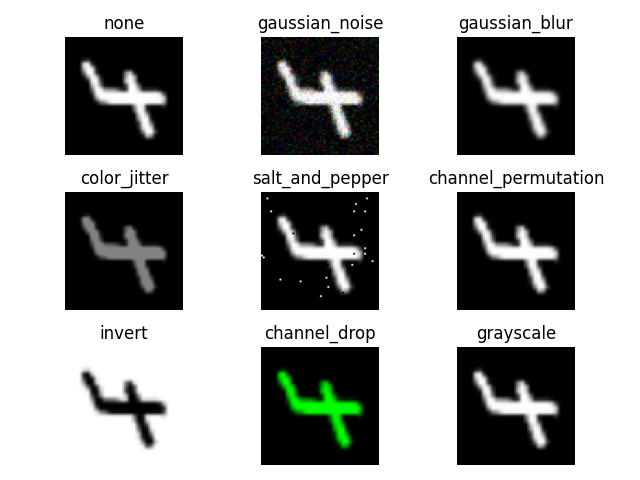
\includegraphics[width=0.48\textwidth]{images/mnist_perturbations.png}
    \caption{MNIST data with various test perturbations applied}
    \label{mnist_perturbations}
\end{figure}

As seen in the results from \Cref{table1}, the model using our Euclidean distance metric does comparably well with the standard model on most test-time perturbations. Its accuracy suffers most notably on the Gaussian noise perturbation. We also see that our proposed method performs much better on the inversion perturbation. The learned mapping model, on the other hand, has a significantly reduced accuracy on nearly all the tested perturbations, likely because it has only learned the training set's color distribution of grayscale pixels. This small color variation within the training set causes the learned mapping model to overfit the color distribution, and it may consider pixels with new colors as out-of-distribution.

\begin{table}[h!]
    \centering
    \begin{tabular}{||c | c c c||}
        \hline
        Perturbations       & Normal         & Euclidean      & Learned \\ [0.5ex]
        \hline\hline
        None                & \textbf{99.17} & 98.50          & 96.59   \\
        Gaussian Noise      & \textbf{98.78} & 90.05          & 75.49   \\
        Gaussian Blur       & \textbf{98.84} & 94.80          & 95.70   \\
        Color Jitter        & \textbf{98.39} & 92.54          & 91.67   \\
        Salt And Pepper     & \textbf{98.46} & 97.12          & 92.86   \\
        Channel Permutation & \textbf{99.17} & 98.50          & 96.59   \\
        Invert              & 9.91           & \textbf{98.46} & 87.60   \\
        Channel Drop        & 77.81          & \textbf{91.04} & 84.59   \\
        Grayscale           & \textbf{99.18} & 98.53          & 96.48   \\
        \hline
        Average             & 86.63          & \textbf{95.50} & 90.84   \\
        \hline
    \end{tabular}
    \caption{ResNet-50 models using different convolution layers compared across various test perturbations}
    \label{table1}
\end{table}

We hypothesize that the color invariant layer's difficulty with classification under the Gaussian noise perturbation may be due to the ResNet-50 upsampling the input image from $32\times32$ to $232\times232$. This means each pixel from the MNIST dataset becomes spread out across around a $7\times7$ pixel area in the resized image. Since the ResNet-50's first layer has a kernel size of only 7, the receptive field used for pixel-wise distances may not be useful for the upsampled MNIST images. To test whether this is the case, we perform the same experiment with the LeNet \cite{LeCun98} architecture instead of ResNet-50. Since LeNet uses a kernel size of $4\times4$ directly on the $32\times32$ image, it is able to detect pixel-wise distances across larger areas of the digit. The MNIST classification results using LeNet are shown in \Cref{table2}. As our hypothesis suggested, our model using the Euclidean distance metric improves performance on all tested perturbations when using LeNet and does not suffer as much from the Gaussian noise perturbation.

\begin{table}[h!]
    \centering
    \begin{tabular}{||c | c c c||}
        \hline
        Perturbations       & Normal         & Euclidean      & Learned \\ [0.5ex]
        \hline\hline
        None                & 99.28          & \textbf{99.43} & 82.98   \\
        Gaussian Noise      & 99.05          & \textbf{99.33} & 81.65   \\
        Gaussian Blur       & \textbf{98.17} & 97.83          & 69.14   \\
        Color Jitter        & \textbf{97.61} & 95.87          & 63.56   \\
        Salt And Pepper     & 99.12          & \textbf{99.26} & 79.00   \\
        Channel Permutation & 99.28          & \textbf{99.43} & 82.98   \\
        Invert              & 16.17          & \textbf{99.44} & 80.08   \\
        Channel Drop        & 90.25          & \textbf{97.96} & 29.23   \\
        Grayscale           & 99.28          & \textbf{99.42} & 82.90   \\
        \hline
        Average             & 88.69          & \textbf{98.66} & 72.39   \\
        \hline
    \end{tabular}
    \caption{LeNet models using different convolution layers compared across various test perturbations}
    \label{table2}
\end{table}

\subsection{CIFAR-10 Classification}
We also experiment on the CIFAR-10 dataset using the same ResNet-50 setup described in \Cref{mnistClassification}. In addition to the three models outlined in \Cref{mnistClassification}, we also experiment with training and testing on only grayscale images for the normal model configuration and the model using Euclidean distance color invariance. We add these two models to demonstrate that our method of using pixel-wise distance representation is fundamentally different than just converting an image to grayscale.

The perturbations applied to this dataset can be seen in figure \Cref{cifar_perturbations}. In \Cref{table3}, we observe similar trends from the tests with MNIST.  The normal models operating in both the RGB and grayscale color spaces struggle with the color inversion perturbation, while the pixel-wise distance based models struggle with the Gaussian noise and blurring perturbations. Given the larger variety of colors, we find the model using the learned mapping cosine similarity distance metric performs much better with respect to other models than when tested on MNIST.

\begin{table*}
    \centering
    \begin{tabular}{|| c | c c c | c c ||}
        \hline
                            & \multicolumn{3}{| c |}{RGB} & \multicolumn{2}{| c ||}{grayscale}                                     \\
        Perturbations       & Normal                      & Euclidean                          & Learned & Normal & Euclidean      \\ [0.5ex]
        \hline\hline
        None                & \textbf{82.25}              & 79.31                              & 76.55   & 78.78  & 78.83          \\
        Gaussian Noise      & \textbf{62.59}              & 16.10                              & 15.39   & 47.94  & 26.98          \\
        Gaussian Blur       & \textbf{63.84}              & 57.26                              & 58.64   & 52.25  & 55.71          \\
        Color Jitter        & 62.72                       & 74.24                              & 69.58   & 72.15  & \textbf{74.84} \\
        Salt And Pepper     & \textbf{73.28}              & 71.77                              & 63.18   & 67.00  & 69.56          \\
        Channel Permutation & 69.00                       & \textbf{79.31}                     & 75.22   & 79.02  & 78.77          \\
        Invert              & 38.83                       & \textbf{79.32}                     & 73.21   & 52.24  & 78.85          \\
        Hue Shift           & 68.99                       & \textbf{79.20}                     & 75.03   & 78.59  & 78.68          \\
        Grayscale           & 73.50                       & 76.65                              & 71.67   & 78.80  & \textbf{78.83} \\
        \hline
        Average             & 66.11                       & 68.13                              & 64.27   & 67.42  & \textbf{69.01} \\
        \hline
    \end{tabular}
    \caption{We show the classification accuracy of ResNet-50 models using different convolution layers compared across various test perturbations. Models under RGB were trained on the standard RGB images and tested with the perturbations applied directly to the RGB images. Models under grayscale were trained with grayscale images and tested on perturbations applied after the RGB images were converted to grayscale}
    \label{table3}
\end{table*}

\begin{figure}[h!]
    \centering
    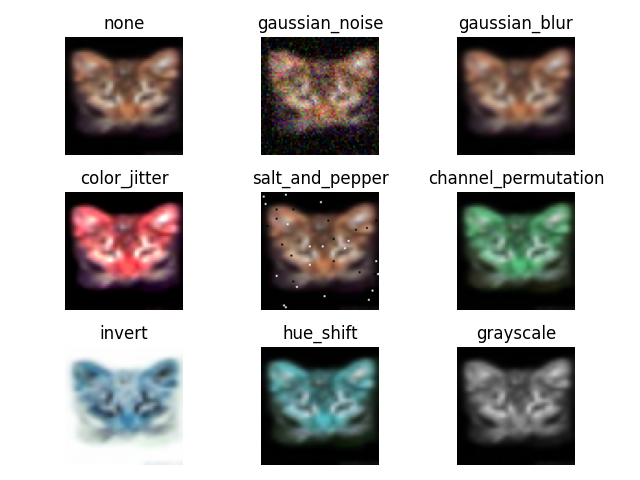
\includegraphics[width=0.48\textwidth]{images/cifar10_perturbations.png}
    \caption{CIFAR-10 data with various test perturbations applied}
    \label{cifar_perturbations}
\end{figure}

To investigate how the mapping model learns to separate images, we uniformly sample from the RGB cube and pass the RGB values through the mapping model. With the representations in the embedding space, we perform t-distributed stochastic neighbor embedding (t-SNE) to visualize the color representations in 3-D space as shown in \Cref{3d_embedding}. Surprisingly, the model seems to learn a linear space of colors between red and blue colors, while finding the largest color difference between black and all other colors. We also see evidence of clustering along this linear space. The importance of these findings requires further experimentation to understand.

\begin{figure}[h!]
    \centering
    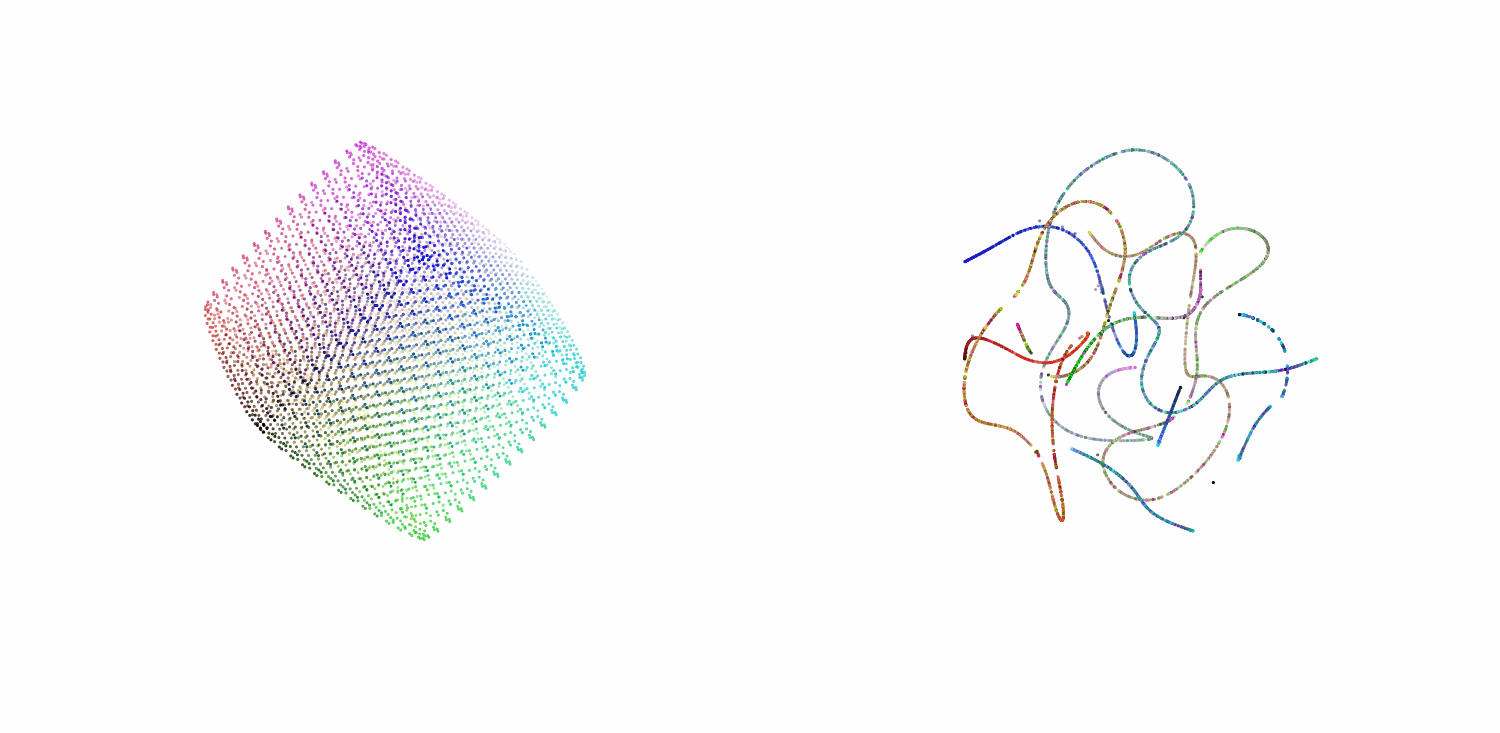
\includegraphics[width=0.48\textwidth]{images/embedding.png}
    \caption{3D t-SNE embedding of the RGB cube (left) and learned colorspace mapping (right).}
    \label{3d_embedding}
\end{figure}

\subsection{Image Generation}
For our GAN setup, we used the DCGAN architecture \cite{radford} with a generator learning rate of 0.0003 and discriminator learning rate of 0.00005. To enforce color invariant generation, we attempt to generate the pixel-wise distance image representations directly rather than RGB images. For our pixel-wise distance representations, we set the receptive field hyperparameter to a size of $9\times9$. This means the layers of the GAN which deal with the image directly increase their channels to 81, meaning each pixel's color difference between itself and its neighbors up to 4 pixels away is included. Using the generated pixel-wise distance image representations, we then visualize the images using our colorization algorithm with random seeding.

Initially, we attempt to generate images based on the CIFAR-10 dataset. This distribution of images proves too challenging for the GAN to learn. We attribute this GAN failure to the complexity of the dataset. While our bias towards color invariance may mitigate having to search the entire color space during model training, we believe our models trade this challenge for a different problem: searching over the shape, size, and pose space each object can take. We believe that given further tuning and adjstment, a color invariant model could learn this dataset effectively.

However, given that the CIFAR-10 dataset's distribution contains complicated objects with a wide intra-class range of shapes, poses, and camera distances, we pivot to experimenting with generating CelebA images. The CelebA dataset is more amenable to being modeled using only the pixel-wise distance representation because the distribution of faces does not have a wide range of shapes, angles, or distances. Using DCGAN, we were able to generate the images shown in \Cref{celeba}.

\begin{figure}[h!]
    \centering
    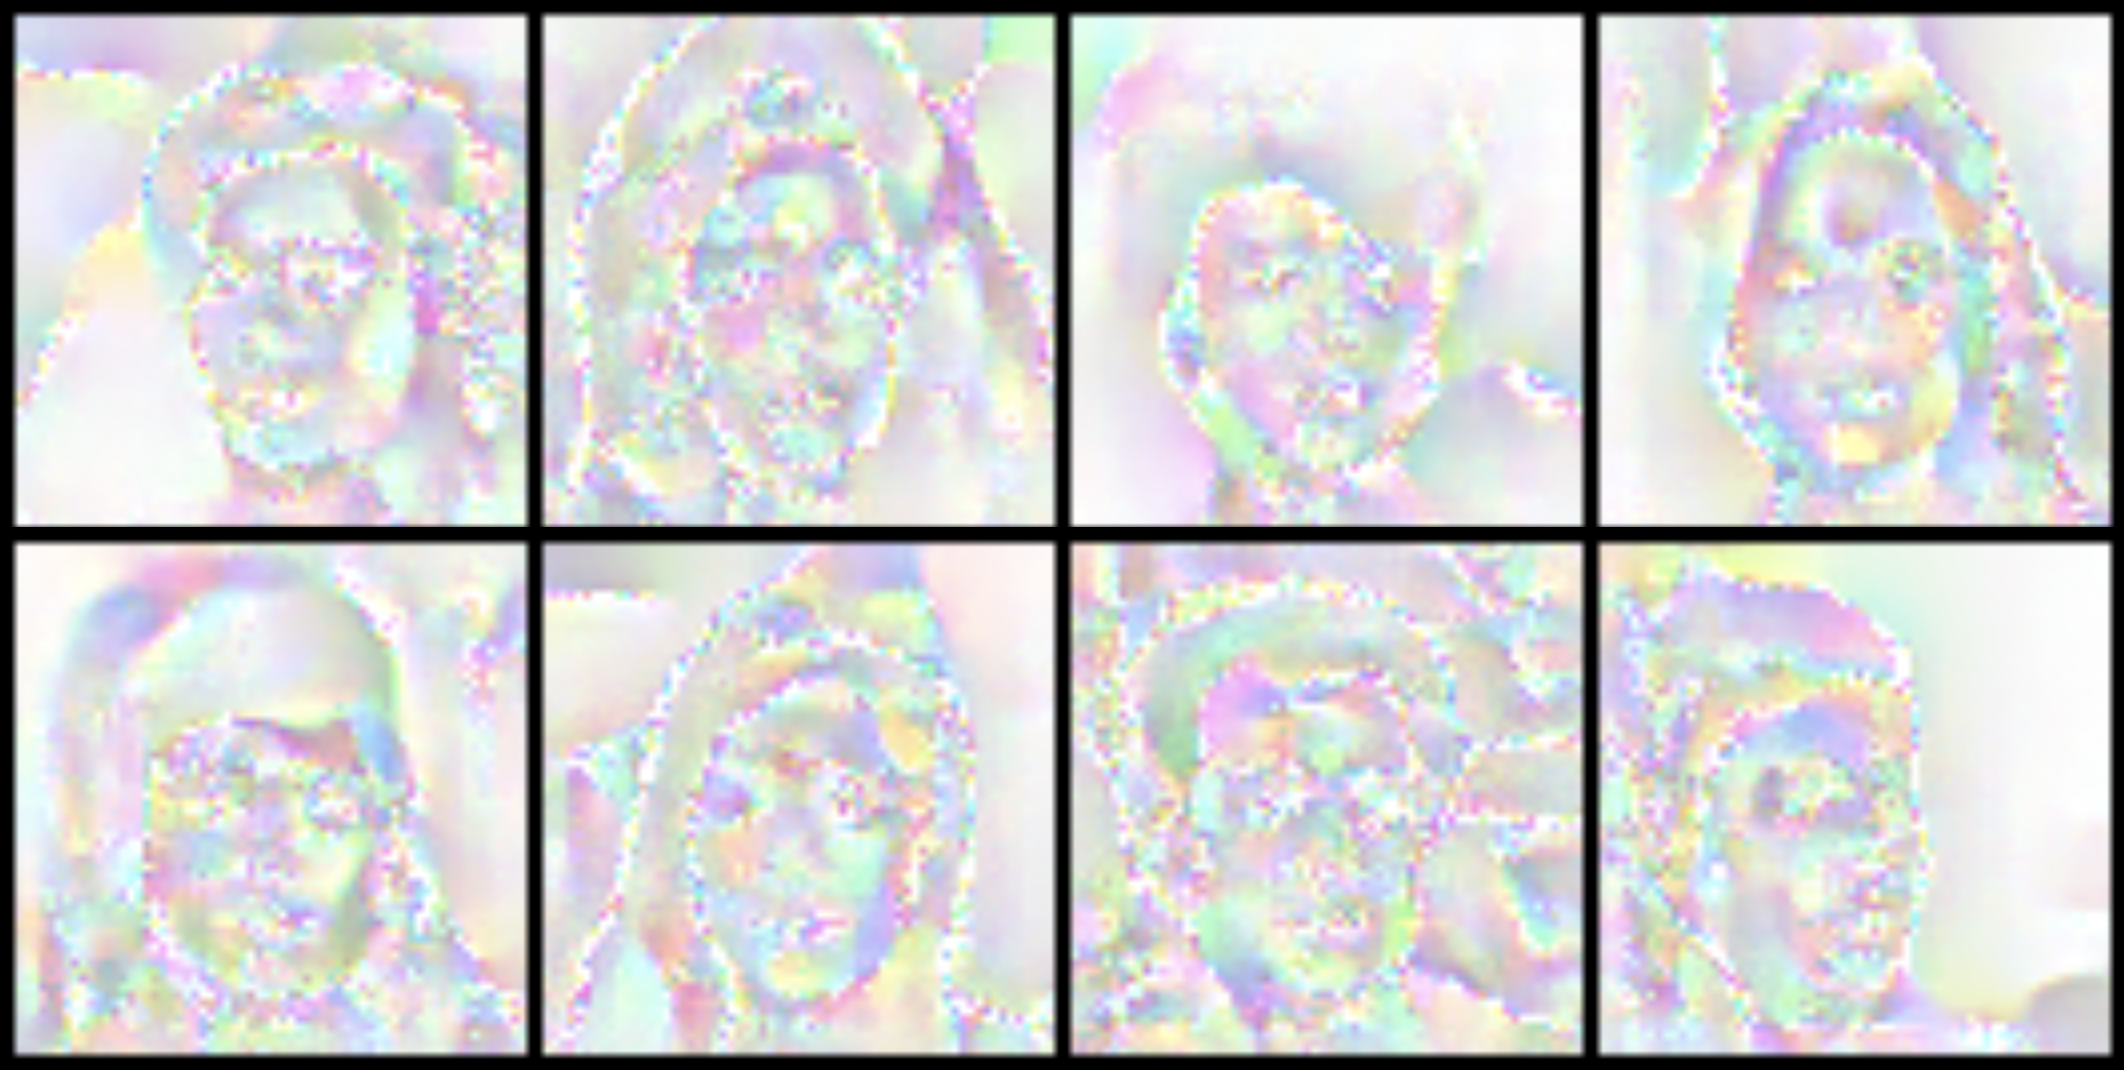
\includegraphics[width=0.48\textwidth]{images/ganGrid.png}
    \caption{Generated CelebA images with solid white seeding during colorization}
    \label{celeba}
\end{figure}

From these generated images, we can see that the color invariant version of DCGAN learns features such as face outlines, hair outlines, and eyes. The images in \Cref{celeba} use solid white seeding during colorization, but a user can also use our proposed biased pixel seeding to choose colorization preferences such as hair, skin, and eye color. This method of colorization is demonstrated in \Cref{recolorization_grid} parts (d) and (e).

\section{Conclusions}

Using our proposed layer for color invariance, we are able to generalize better than normal convolution layers to unseen color distributions during image classification. This reduces the amount of augmentations needed during training and is especially well suited for datasets which are likely to overfit to certain color distributions. However, this bias toward color invariance introduces a new challenge of noise perturbations and object orientation diversity. An example of a dataset well suited for our method is biomedical images, which are taken from a fixed angle and magnification. Models trained on slide-tissue images may overfit to the stain color distribution used in the training set when using standard convolution layers, but could mitigate this issue with a color invariant convolution layer.

Even though our work has demonstrated the ability of convolutional neural networks to classify images without direct color information, our method also allows the pixel-wise gradient representation layer to function alongside its standard RGB counterpart.

During image synthesis, we find that using a self attention image representation to guide colorization allows users to have more control over specific object colors. While our method's runtime is slower than a standard GAN due to the iterative algorithm, this technique allows better object-color disentanglement.

\section{Future Work}

There are many future works researchers can explore using pixel-wise distance representations for color invariant image classification and synthesis. The color invariant GAN we propose could be used as a data augmentation technique for supervised and unsupervised learning tasks to force new models to learn decision boundaries which are less biased toward object color and texture. However, we are more excited by the prospects this idea poses for avoiding the need to use color changes for data augmentation altogether.

To expand upon classification models, we would like to compare our color invariant layer's performance when applied to state of the art models trained using color augmentation techniques. This may highlight any color biases contained within recent models, but the effects will likely be harder to detect. Additionally, we would like to find a distance metric that better aligns with human perception. This could take the form of color clustering or may even be as simple as converting RGB to LAB before calculating the Euclidean distance between pixels, as LAB was designed to represent perceptual distances between colors in Euclidean space. It is possible that with further tuning of the model and given more training time and/or resources, the impact of the colorspace would become clear particularly when comparing RGB to LAB.

As mentioned in \Cref{colorInvariant}, we are also interested in applying this method to vision transformers since the self attention representation is inspired by the key-query section of the transformer block. Given that our method also allows the pixel-wise distance representation layer to be utilized alongside its standard RGB counterpart, we are also interested in testing whether using both layers could function better than either method alone. With one layer biased towards color and the other towards shape, a classification model implementing both may get the benefits or drawbacks of both.

Given the challenges modeling the CIFAR-10 dataset, we would like to explore generating more datasets to get a better intuition of what can and cannot be learned by a GAN with color invariance.

To further improve the colorization algorithm, we propose weighting the pixel updates based on inverse color proximity during backpropagation. This is because there is less variation and therefore more confidence when determining a pixel's value with smaller Euclidean distance from another pixel. There are many other possible improvements on colorization algorithms that could produce more realistic results without introducing color bias from a training dataset. One idea is allowing a colorization algorithm to have access to some information about lightness so that it would maintain the realism of shadowed and brightly lit portions of an image as it colors them. Additionally, providing object masking information would be one way for the colorization algorithm to maintain color continuity in the colorization of single objects without introducing bias.

    {\small
        \bibliographystyle{ieee_fullname}
        \bibliography{bibliography}
    }

\end{document}
